\let\negmedspace\undefined
\let\negthickspace\undefined
\documentclass[journal,12pt,onecolumn]{IEEEtran}
\usepackage{cite}
\usepackage{amsmath,amssymb,amsfonts,amsthm}
\usepackage{algorithmic}
\usepackage{graphicx}
\usepackage{textcomp}
\usepackage{xcolor}
\usepackage{txfonts}
\usepackage{listings}
\usepackage{enumitem}
\usepackage{mathtools}
\usepackage{gensymb}
\usepackage{gvv}
\usepackage{tkz-euclide} % loads  TikZ and tkz-base
\usepackage{listings}
\usepackage{circuitikz}
\begin{document}
\title{Gate Assignment}
\author{SAMMETA SAIPOORNA\\ EE23BTECH11055}
\maketitle
% Define variables for the arithmetic progression
\textbf{Question}

The voltage source \( V_s = 10\sqrt{2} \sin(20000\pi t) \) V has an internal resistance of \( 50 \) ohms. The RMS value of the current through \( R \) is \_\_\_ (in mA) (rounded off to one decimal place).\\
\begin{center}
\begin{circuitikz}
        \draw (0,0) to [vsourcesin,l=$V_s$] (0,2)
                    to [R,l=$25\Omega$] (4,2)
                    to [L,l=$\frac{1}{20\pi}\text{mH}$] (4,0)
                    to [C,l=$\frac{1}{20\pi}\text{mF}$] (0,0)            
    \end{circuitikz}

\end{center}
\hfill(GATE IN 2023)\\
\textbf{Solution:}


\begin{table}[htbp]
\centering
\begin{tabular}{|c|c|}
\hline
\textbf{Parameter} & \textbf{Value} \\
\hline
$V_s$ & $10\sqrt{2} \sin(20000\pi t)$ V \\
$R$ &  $??$ \\
$R_{\text{internal}}$ & 50 ohms \\
$R_{\text{net}}$ & $R$ + $R_{\text{internal}}$ \\
\omega & 20000\pi\\
\hline
\end{tabular}
\caption{Input Parameters}
\label{tab:parameters}
\end{table}

\begin{align}
    V(s) &= Z I(s) \\
    \frac{V(s)}{I(s)} &= Z = R + R_{\text{internal}} + Ls + \frac{1}{Cs} \\
    &= 50 + 25 + \frac{s}{20000\pi} + \frac{20000\pi}{s} \\
    V_{\text{RMS}} &= \frac{10\sqrt{2}}{\sqrt{2}} = 10 \, \text{V} \\
    \text{Putting } s &= j\omega \\
    \frac{V(j\omega)}{I(j\omega)} &= |Z| \cdot e^{\angle Z} \\
    &= 75 + \frac{20000 \pi j}{20000 \pi} + \frac{20000\pi }{20000 \pi j} \\
    &= 75 + j - j \\
    &=75 \\
    I_{\text{RMS}} &= \frac{V_{\text{RMS}}}{|Z|}  \\
    &= \frac{10}{75} \times 1000 = \frac{2000}{15} \approx 133.3 \, \text{mA}
\end{align}
\begin{figure}[h!]
    \centering
    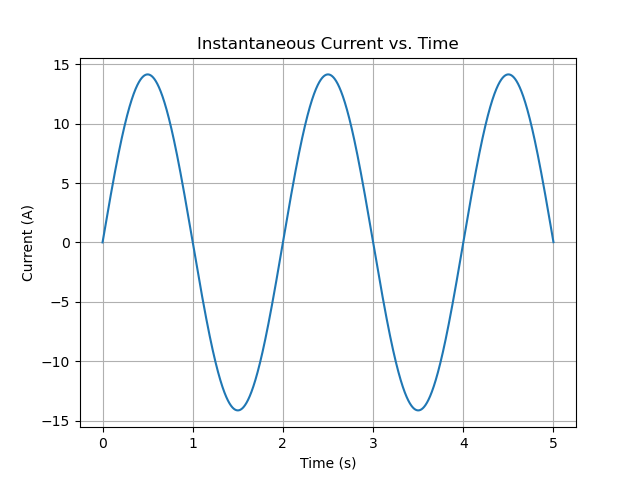
\includegraphics[width=\columnwidth]{figs/gate1.png}    
\end{figure}

\end{document}

